\documentclass{article}
\usepackage[english, greek]{babel} 
\usepackage[utf8]{inputenc} % Required for inputting international characters
\usepackage[T1]{fontenc} % Output font encoding for international characters
\title{thesis_summary}

\usepackage{graphicx}
\usepackage{float}
\usepackage{caption}
\usepackage{subcaption}

\usepackage{amsmath}

\graphicspath{ {images/} }

\usepackage[autostyle=true]{csquotes} % Required to generate language-dependent quotes in the bibliography
\MakeOuterQuote{"}
\def\e{\selectlanguage{english}} % define convenience shortcut for changing language
\def\g{\selectlanguage{greek}}

\begin{document}

   \begin{center}
      \Large\textbf{Στερεοσκοπική όραση με χρήση τεχνητού νευρωνικού δικτύου}
      \\
      \vspace*{3mm}
      \large\textit{Βασίλης Γκολέμης}
      \\
      \vspace*{3mm}
      \large\textit{10/11/2017}
   \end{center}
   \vspace*{5mm}

\section{Περιγραφή προβλήματος}

Η στερεοσκοπική υπολογιστική όραση προσομοιάζει την μέθοδο με την οποία το μεγαλύτερο μέρος των ζωντανών οργανισμών (αναμεσά τους και ο άνθρωπος) αντιλαμβάνονται το τρισδιάστατο περιβάλλον. Ως πληροφορία εισόδου δεχόμαστε δύο λήψεις σε στερεοσκοπική διάταξη, όπως φαίνεται στην εικόνα \ref{fig:stereo_cameras}. Τα σημεία που ανήκουν εντός του οπτικού πεδίου και των δύο λήψεων, ακολουθούν την σχέση

\begin{equation} 
	z = \dfrac{fB}{x_R-x_L} = \dfrac{fB}{d}
    \label{eq:disp2depth}
\end{equation}

Τα μεγέθη της σχέσης \ref{eq:disp2depth} αποτυπώνονται στην εικόνα \ref{fig:stereo_geometry}. Συμπερασματικά, από το πόσο μετατοπισμένο κατά τον οριζόντιο άξονα (μέγεθος $d = x_R-x_L$) εμφανίζεται κάθε σημείο της εικόνας αναφοράς αντιλαμβανόμαστε πόσο κοντά/μακριά είναι από το πέτασμα της κάμερας (αντιστρόφως ανάλογα).Για παράδειγμα, ο ουρανός που βρίσκεται πάρα πολύ μακριά από τις κάμερες ($z \rightarrow \infty$) θα αποτυπωθεί στο ίδιο σημείο (ίδια τετμημένη) και στις δύο λήψεις ($d = x_R-x_L \rightarrow 0$). Τα μεγέθη $f,b$ είναι σταθερές που περιγράφουν τη στερεοσκοπική διάταξη.

Επομένως, για την επίλυση του προβλήματος οφείλουμε να αντιστοιχήσουμε κάθε σημείο της εικόνας αναφοράς στο "αντίστοιχο" σημείο που αποτυπώθηκε στην έτερη λήψη. Η ακρίβεια με την οποία θα επιτευχθεί αυτή η "αντιστοίχηση" προσδιορίζει την ποιότητα της λύσης.

\begin{figure}
	\centering
    \begin{subfigure}{0.5\textwidth}
    	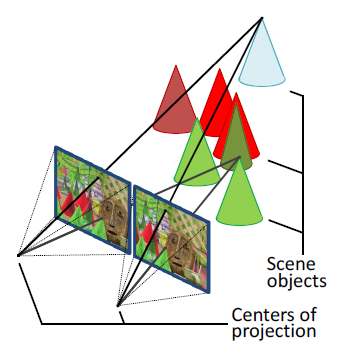
\includegraphics[scale=0.4]{stereo_cameras.png}
    	\caption{Παράδειγμα στερεοσκοπικής λήψης}
    	\label{fig:stereo_cameras}
    \end{subfigure}
    \begin{subfigure}{0.49\textwidth}
        \centering
        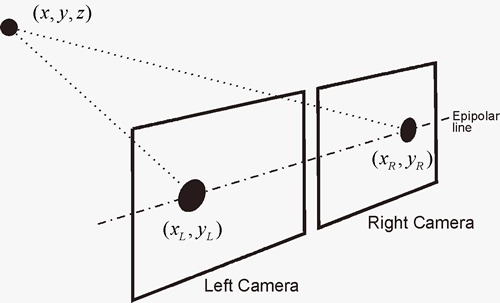
\includegraphics[scale=0.4]{stereo_geometry.jpg}
        \caption{Στερεοσκοπική γεωμετρία}
        \label{fig:stereo_geometry}
    \end{subfigure}
\end{figure}



\section{Επίλυση του προβλήματος}

Βασισμένοι σε πρόσφατη βιβλιογραφία, προσσεγγίσαμε το πρόβλημα της "αντιστοίχησης" με χρήση τεχνητού συνελικτικού νευρωνικού δικτύου, έναν εξειδικευμένο αλγόριθμο μηχανικής μάθησης σε εικόνες.
Στόχος του αλγορίθμου είναι η εκμάθηση από παραδείγματα της σύγκρισης δύο σημείων κι η επιστροφή μιας τιμής (σκορ) ομοιότητας. Αν τα δύο σημείο είναι "αντίστοιχα" (αποτυπώνουν το ίδιο τρισδιάστατο σημείο στην κάθε λήψη) επιθυμούμε το σκορ να μεγιστοποιείται. Αντιθέτως, για δύο τυχαία (αναντίστοιχα) σημεία επιθυμούμε το σκορ να είναι μικρό.
Η σύγκριση δύο σημείων γίνεται συγκρίνοντας τις τετράγωνες περιοχές που τα περιβάλλουν (γειτονιές).

Για την εκμάθηση αυτής της διαδικασίας χρησιμοποιήθηκαν οι πιο γνωστές συλλογές εικόνων \e KITTI 2012, KITTI 2015 \g και \e Middlebury. \g Οι συλλογές αυτές περιέχουν την πραγματική πληροφορία μετατόπισης κάθε σημείου μετρημένη με κατάλληλα εργαλεία, όπως για παράδειγμα το \e lidar. \g

Η αρχιτεκτονική του νευρωνικού δικτύου που δημιουργήσαμε φαίνεται στο σχήμα \ref{fig:neural_net_arch}. Υπάρχουν 9 συνελικτικά επίπεδα, υπεύθυνα για την εξαγωγή του κατάλληλου διανύσματος χαρακτηριστικών \e (feature vector) \g κάθε γειτονιάς και μια πράξη εσωτερικού γινομένου υπολογίζει την τιμή ομοιότητας.

\begin{figure}
	\centering
    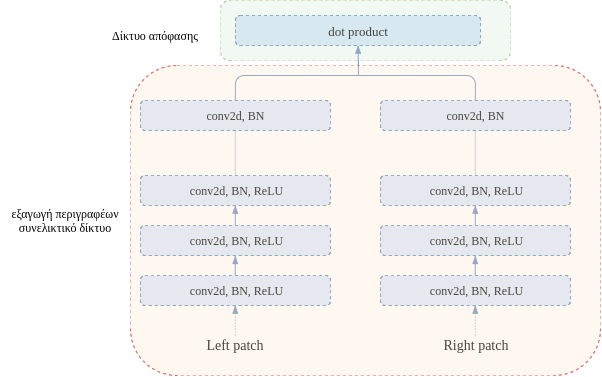
\includegraphics[scale=0.6]{neural_net_arch.png}
    \caption{Αρχιτεκτονική νευρωνικού δικτύου}
    \label{fig:neural_net_arch}
\end{figure}

Η σύγκριση κάθε σημείου της εικόνας αναφοράς με κάθε πιθανή θέση που μπορεί να αποτυπώθηκε στην έτερη λήψη δημιουργεί τον πίνακα ομοιότητας $C_{init}(x,y,d)$. Ακολούθως εφαρμόζουμε τις τεχνικές εξομάλυνσης και βαλτίωσης του αποτελέσματος \e cross-based cost aggregation, semi-global matching \g και \e left-right consistency check. \g Τα βήματα αυτά δημιουργούν έναν βελτιωμένο πίνακα ομοιότητας $C_{refined}(x,y,d)$. Από αυτόν τον πίνακα επιλέγεται για κάθε σημείο $(x,y)$ η θέση με την μέγιστη ομοιότητα.

\section{Αποτελέσματα}

Συγκεντρωτικά αποτελέσματα της μεθόδου μας φαίνονται στον πίνακα \ref{tbl:results}. Ακολούθως φαίνεται ένα ενδεικτικό παράδειγμα εφαρμογής της μεθόδου. 

\begin{table}[t]

\centering
\begin{tabular}{l|c}
\multicolumn{2}{c}{\textbf{\e KITTI 2012 \g}} \\ \hline 
Μέσο σφάλμα & $5.787\%$\\
Μέσο σφάλμα απόστασης & $1.357 \mathbf{px}$\\
\multicolumn{2}{c}{\textbf{\e KITTI 2015 \g}} \\ \hline 
Μέσο σφάλμα & $6.545\%$\\
Μέσο σφάλμα απόστασης & $1.577 \mathbf{px}$\\	
\multicolumn{2}{c}{\textbf{\e Middlebury \g}} \\ \hline 
Μέσο σφάλμα & $9.475\%$\\
Μέσο σφάλμα απόστασης & $2.144 \mathbf{px}$\\	

\end{tabular}
\caption{Συνοπτικός πίνακας αποτελεσμάτων.}
\label{tbl:results}
\end{table}

\begin{figure}
	\centering
	\begin{subfigure}{1\textwidth}
		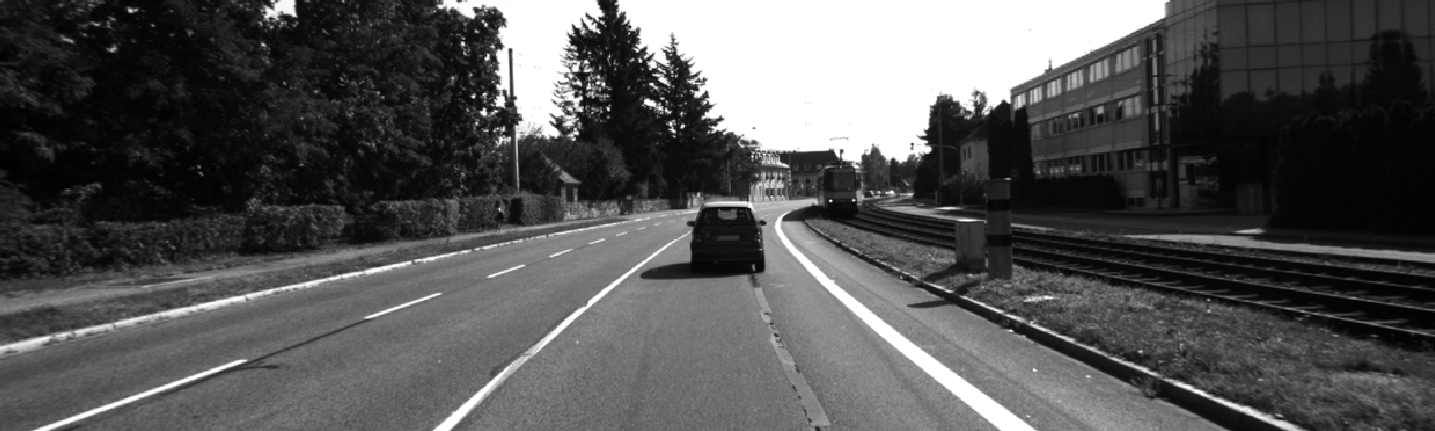
\includegraphics[width=\textwidth]{kitti2015_best_imL.png}
        \caption{Εικόνα αναφοράς.}
	\end{subfigure}
	
	\begin{subfigure}{1\textwidth}
		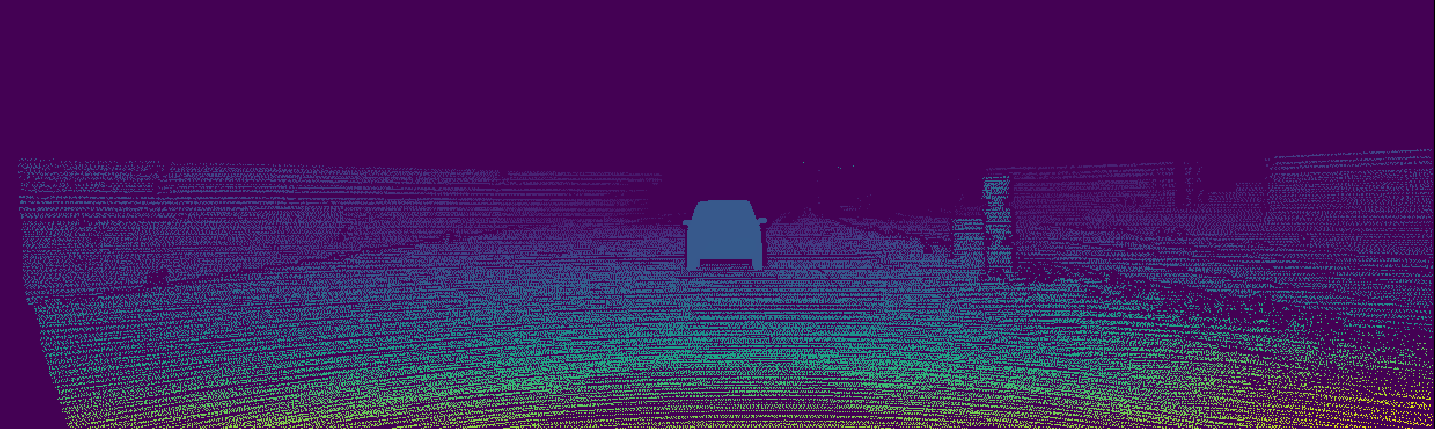
\includegraphics[width=\textwidth]{kitti2015_best_disparity_gt.png}
        \caption{Πραγματική πληροφορία βάθους, όπως μετρήθηκε μέσω \e lidar. \g}
	\end{subfigure}
	
	\begin{subfigure}{1\textwidth}
		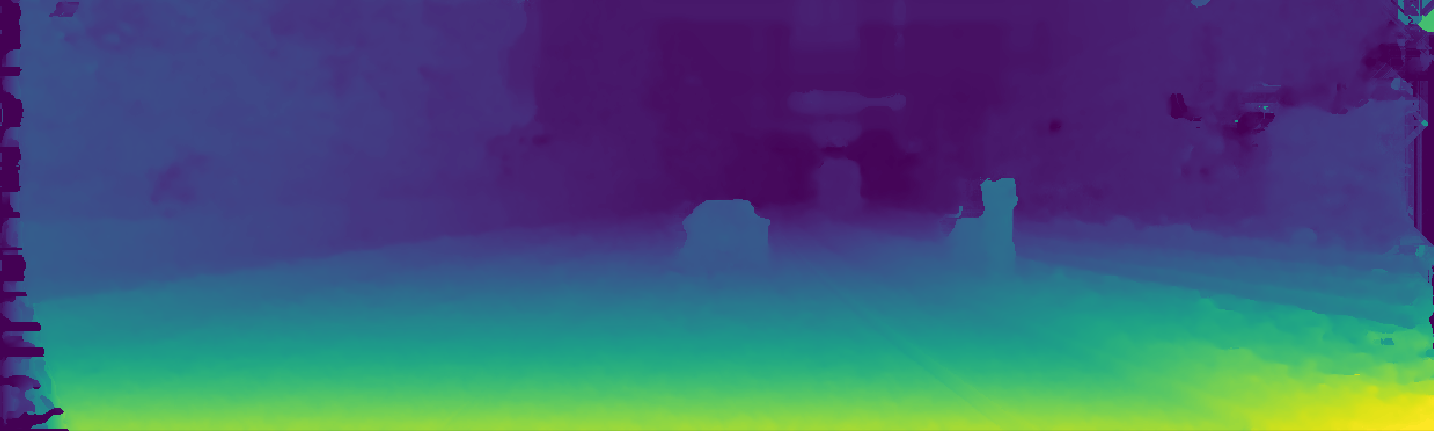
\includegraphics[width=\textwidth]{kitti2015_best_disparity_pred.png}
        \caption{Πρόβλεψη πληροφορίας βάθους από την μέθοδό μας.}
	\end{subfigure}
	
	\caption{Ενδεικτικό παράδειγμα.}
	\label{fig:kitti2015_best_example}
\end{figure}

\e
\nocite{*}
\bibliographystyle{plain}
\bibliography{bibliography}
\g

\end{document}
